%% Ein einfaches Template für einen Übungsbericht unter Verwendung des Hagenberg
%% Setups, basierend auf der LaTeX 'report' Standardklasse.
%%% äöüÄÖÜß  <-- keine deutschen Umlaute hier? UTF-faehigen Editor verwenden!

%%% Magic Comments zum Setzen der korrekten Parameter in kompatiblen IDEs
% !TeX encoding = utf8
% !TeX program = pdflatex
% !TeX spellcheck = de_DE
% !BIB program = biber

\documentclass[german,notitlepage,smartquotes]{hgbreport}
% Zulässige Optionen in [..]:
%    Hauptsprache: 'german' (default), 'english'
%    Option zur Umwandlung in typografische Anführungszeichen: 'smartquotes'
%    APA Zitierstil: 'apa'
%    Erzeuge keine separate Titelseite: 'notitlepage'
%%%-----------------------------------------------------------------------------

\RequirePackage[utf8]{inputenc} % bei Verw. von lualatex oder xelatex entfernen!

\renewcommand{\chapter}[1]{} % Deaktiviere den \chapter Befehl
\graphicspath{{images/}}     % Verzeichnis mit Bildern und Grafiken
\bibliography{references}    % Biblatex-Literaturdatei (references.bib)
\ExecuteBibliographyOptions{backref=false} % Keine Rückreferenzen bei Quellen

%%%-----------------------------------------------------------------------------
\setcounter{chapter}{3}	% <----- Auf die Übungsnummer setzen
%%%-----------------------------------------------------------------------------

\author{Julian Jany}                        % Name
\title{BVA2 Fortgeschrittene Bildverarbeitung und -analyse -- SS 2022\\ % Name der Übung
				Übungsabgabe \arabic{chapter}}
\date{\today}

%%%-----------------------------------------------------------------------------
\begin{document}
%%%-----------------------------------------------------------------------------
\maketitle
%%%-----------------------------------------------------------------------------

%\begin{abstract}\noindent
%\ldots
%\end{abstract}

%%%-----------------------------------------------------------------------------

\section{Richardson Lucy Deconvolution}

\subsection{Problembeschreibung}

Es soll ein \texttt{ImageJ Plugin} entwickelt werden. 
Das Plugin soll den iterativen Algorithmus \textit{Richardson Lucy Deconvolution} anwenden, und damit ein \zB unscharfes Bild "scharfstellen" können. 

\subsection{Lösungsbeschreibung}

\subsection{Implementierung}

Hier werden interessante Code-Teile der Implementierung inkludiert.

\subsubsection{Extraktion der Buchstaben}

\begin{program}[h]
\caption{\texttt{splitLine(...)}}
\label{prog:extract-01}
\begin{JavaCode}
public Vector<SubImageRegion> splitLine(int[][] inImg, int width, int height, int BG_val, int FG_val) {
	boolean insideEmptyRegion = isEmptyRow(inImg, width, 0, BG_val);
	int lineRowStart = 0;
	Vector<SubImageRegion> rows = new Vector<>();

	for (int curRow = 1; curRow < height; curRow++) {
		if (insideEmptyRegion != isEmptyRow(inImg, width, curRow, BG_val)) {
			if (insideEmptyRegion) {
				lineRowStart = curRow;
			} else {
				rows.add(new SubImageRegion(0, lineRowStart, width, curRow - lineRowStart, inImg));
			}
			insideEmptyRegion = !insideEmptyRegion;
		}
	}

	return rows;
}
\end{JavaCode}
\end{program}

\begin{program}[h]
\caption{\texttt{shrinkCharVertically(...)}}
\label{prog:extract-02}
\begin{JavaCode}
public SubImageRegion shrinkCharVertically(SubImageRegion charImg, int BG_val) {
	int lineRowStart = 0;
	boolean insideEmptyRegion = isEmptyRow(charImg.subImgArr, charImg.width, lineRowStart, BG_val);
	if (insideEmptyRegion) {
		lineRowStart++;
		while (lineRowStart < charImg.height && isEmptyRow(charImg.subImgArr, charImg.width, lineRowStart, BG_val)) {
			lineRowStart++;
		}
	}

	int lineRowEnd = charImg.height - 1;
	insideEmptyRegion = isEmptyRow(charImg.subImgArr, charImg.width, lineRowEnd, BG_val);
	if (insideEmptyRegion) {
		lineRowEnd--;
		while (lineRowEnd >= 0 && isEmptyRow(charImg.subImgArr, charImg.width, lineRowEnd, BG_val)) {
			lineRowEnd--;
		}
	}

	SubImageRegion shrunk = new SubImageRegion(0, lineRowStart, charImg.width, lineRowEnd - lineRowStart + 1, charImg.subImgArr);
	shrunk.startX = charImg.startX;
	shrunk.startY = charImg.startY + lineRowStart;
	return shrunk;
}
\end{JavaCode}
\end{program}

\begin{program}[h]
\caption{\texttt{splitCharactersVertically(...)}}
\label{prog:extract-03}
\begin{JavaCode}
public Vector<SubImageRegion> splitCharactersVertically(SubImageRegion rowImage, int BG_val) {
	boolean insideEmptyRegion = isEmptyColumn(rowImage.subImgArr, rowImage.height, 0, BG_val);
	int lineColStart = 0;
	Vector<SubImageRegion> cols = new Vector<>();

	for (int curCol = 1; curCol < rowImage.width; curCol++) {
		if (insideEmptyRegion != isEmptyColumn(rowImage.subImgArr, rowImage.height, curCol, BG_val)) {
			if (insideEmptyRegion) {
				lineColStart = curCol;
			} else{
				SubImageRegion col = new SubImageRegion(lineColStart, 0, curCol-lineColStart, rowImage.height, rowImage.subImgArr);
				col.startY = rowImage.startY;
				cols.add(
						shrinkCharVertically(col, BG_val));
			}
			insideEmptyRegion = !insideEmptyRegion;
		}
	}

	return cols;
}
\end{JavaCode}
\end{program}

\begin{program}[h]
\caption{\texttt{splitCharacters(...)}}
\label{prog:extract-04}
\begin{JavaCode}
public Vector<Vector<SubImageRegion>> splitCharacters(int[][] inImg, int width, int height, int BG_val, int FG_val) {
	Vector<Vector<SubImageRegion>> returnCharMatrix = new Vector<Vector<SubImageRegion>>();

	Vector<SubImageRegion> lines = splitLine(inImg, width, height, BG_val, FG_val);
	for (SubImageRegion line : lines) {
		returnCharMatrix.add(
				splitCharactersVertically(line, BG_val));
	}

	return returnCharMatrix;
}
\end{JavaCode}
\end{program}

\clearpage

\subsubsection{Referenzbestimmung}

\begin{program}[h]
\caption{\texttt{calcFeatureArr(...)}}
\label{prog:calc-feature-arr}
\begin{JavaCode}
double[] calcFeatureArr(SubImageRegion region, int FGval, Vector<ImageFeatureBase> featuresToUse) {
	double[] featureResArr = new double[featuresToUse.size()];
	int idx = 0;
	for (ImageFeatureBase ifb : featuresToUse) {
		featureResArr[idx] = ifb.CalcFeatureVal(region, FGval);
		idx++;
	}
	return featureResArr;
}
\end{JavaCode}
\end{program}

\begin{program}[h]
\caption{\texttt{ImageFeature: Circularity}}
\label{prog:img-feature-circularity}
\begin{JavaCode}
class ImageFeature_Circularity extends ImageFeatureBase {
	public ImageFeature_Circularity() {
		this.description = "circularity";
	}

	@Override
	public double CalcFeatureVal(SubImageRegion imgRegion, int FG_val) {
		final int scaleFactor = (int)Math.ceil(128. / imgRegion.width);
		int[][] upscaledImg =
				SubImageRegion.growBorder(
						SubImageRegion.upscale(imgRegion.subImgArr, scaleFactor),
						255-FG_val);
		int[][] perimeterImg = SubImageRegion.dilateAndSubtract(upscaledImg, FG_val);

		int area = SubImageRegion.foregroundPixelCount(upscaledImg, FG_val);
		int perimeter = SubImageRegion.foregroundPixelCount(perimeterImg, FG_val);

		return (4. * Math.PI * (double)area) / ((double)perimeter*(double)perimeter);
	}
}
\end{JavaCode}
\end{program}

\begin{program}[h]
\caption{\texttt{upscale(...)}}
\label{prog:upscale}
\begin{JavaCode}
public static int[][] upscale(int[][] img, int scaleFactor) {
	final int width = img.length;
	final int height = img[0].length;
	final int newWidth  = width * scaleFactor;
	final int newHeight = height * scaleFactor;
	int[][] upscaledArr = new int[newWidth][newHeight];

	for (int x = 0; x < width; x++) {
		for (int y = 0; y < height; y++) {
			for (int xOff = 0; xOff < scaleFactor; xOff++) {
				for (int yOff = 0; yOff < scaleFactor; yOff++) {
					upscaledArr[x*scaleFactor+xOff][y*scaleFactor+yOff] = img[x][y];
				}
			}
		}
	}

	return upscaledArr;
}
\end{JavaCode}
\end{program}

\begin{program}[h]
\caption{\texttt{growBorder(...)}}
\label{prog:grow-border}
\begin{JavaCode}
public static int[][] growBorder(int[][] img, int BG_VAL) {
	final int width = img.length;
	final int height = img[0].length;
	final int newWidth  = width + 2;
	final int newHeight = height + 2;
	int[][] borderArr = new int[newWidth][newHeight];

	for (int x = 0; x < width; x++) {
		for (int y = 0; y < height; y++) {
			borderArr[x+1][y+1] = img[x][y];
		}
	}

	for (int x = 0; x < newWidth; x++) {
		borderArr[x][0] = BG_VAL;
		borderArr[x][newHeight-1] = BG_VAL;
	}
	for (int y = 0; y < newHeight; y++) {
		borderArr[0][y] = BG_VAL;
		borderArr[newWidth-1][y] = BG_VAL;
	}

	return borderArr;
}
\end{JavaCode}
\end{program}

\begin{program}[h]
\caption{\texttt{dilateAndSubtract(...)}}
\label{prog:dilate-and-subtract}
\begin{JavaCode}
public static int[][] dilateAndSubtract(int[][] img, int FG_VAL) {
	final int width = img.length;
	final int height = img[0].length;
	int[][] dilated = new int[width][height];

	for (int x = 0; x < width; x++) {
		for (int y = 0; y < height; y++) {
			if (img[x][y] == FG_VAL) {
				dilated[x][y] = 255-FG_VAL;
				continue;
			}

			int x_ = x-1;
			int y_ = y;
			if (x_ >= 0 && x_ < width &&
				y_ >= 0 && y_ < height &&
				img[x_][y_] == FG_VAL) {
				dilated[x][y] = FG_VAL;
				continue;
			}
			x_ = x+1;
			y_ = y;
			if (x_ >= 0 && x_ < width &&
				y_ >= 0 && y_ < height &&
				img[x_][y_] == FG_VAL) {
				dilated[x][y] = FG_VAL;
				continue;
			}
			x_ = x;
			y_ = y-1;
			if (x_ >= 0 && x_ < width &&
				y_ >= 0 && y_ < height &&
				img[x_][y_] == FG_VAL) {
				dilated[x][y] = FG_VAL;
				continue;
			}
			x_ = x;
			y_ = y+1;
			if (x_ >= 0 && x_ < width &&
				y_ >= 0 && y_ < height &&
				img[x_][y_] == FG_VAL) {
				dilated[x][y] = FG_VAL;
				continue;
			}
			dilated[x][y] = 255-FG_VAL;
		}
	}

	return dilated;
}
\end{JavaCode}
\end{program}

Die Circularity wird berechnet indem Fläche und Umfang abgeschätzt und dann ins Verhältnis gesetzt werden. Für die Abschätzung des Umfangs wird das Bild des Buchstaben hochskaliert und dann ein Bild der Umrandung berechnet. Die Anzahl der Vordergrung-Pixel dient als Schätzer für dern Umfang.

\begin{figure}[h]
\centering
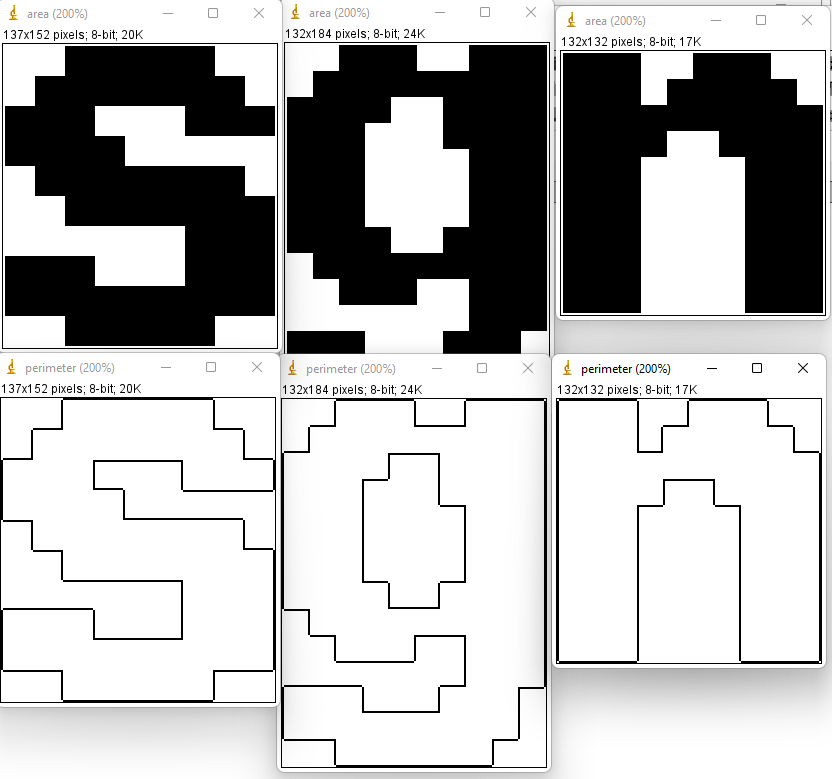
\includegraphics[width=.7\textwidth]{area_perimeter}
\caption{Fläche und Umfang verschiedener beispielhafter Buchstaben.}
\label{fig:area_perimeter}
\end{figure}

\clearpage

\subsubsection{Normalisierung}

\begin{program}[h]
\caption{\texttt{calculateNormArr(...)}}
\label{prog:calc-norm-arr}
\begin{JavaCode}
double[][] calculateNormArr(Vector<Vector<SubImageRegion>> inputRegions, int FGval, Vector<ImageFeatureBase> featuresToUse) {
	double[][] returnVect = new double[featuresToUse.size()][2];
	int featureIdx = 0;
	for(ImageFeatureBase feature : featuresToUse) {
		final double mean = calculateMean(inputRegions, feature, FGval);
		final double sigma = calculateSigma(inputRegions, feature, FGval, mean);
		returnVect[featureIdx][0] = mean;
		returnVect[featureIdx][1] = sigma;
		featureIdx++;
	}
	return returnVect;
}
\end{JavaCode}
\end{program}

\begin{program}[h]
\caption{\texttt{calculateMean(...)}}
\label{prog:calc-mean}
\begin{JavaCode}
double calculateMean(Vector<Vector<SubImageRegion>> inputRegions, ImageFeatureBase feature, int FGval) {
	double sum = 0.0;
	int count = 0;
	// get all extracted chars for calc. of mean
	for(Vector<SubImageRegion> rowVect : inputRegions) {
		for(SubImageRegion charReg : rowVect) {
			double curFeatureVal = feature.CalcFeatureVal(charReg, FGval);
			sum += curFeatureVal;
			++count;
		}
	}
	return sum / count;
}
\end{JavaCode}
\end{program}

\begin{program}[h]
\caption{\texttt{calculateSigma(...)}}
\label{prog:calc-sigma}
\begin{JavaCode}
double calculateSigma(Vector<Vector<SubImageRegion>> inputRegions, ImageFeatureBase feature, int FGval, double mean) {
	double sum = 0.0;
	int count = 0;
	// iterate again for calc. of sigma
	for(Vector<SubImageRegion> rowVect : inputRegions) {
		for(SubImageRegion charReg : rowVect) {
			final double featureDiff = mean - feature.CalcFeatureVal(charReg, FGval);
			sum += (featureDiff*featureDiff);
			++count;
		}
	}
	return Math.sqrt(sum / count);
}
\end{JavaCode}
\end{program}

\subsubsection{Korrelationskoeffizient}

\begin{program}[h]
\caption{\texttt{calcCorrelationCoefficient(...)}}
\label{prog:calc-corr-coeff}
\begin{JavaCode}
double calcCorrelationCoefficient(double[] currFeatureArr, double[] refFeatureArr, double[][] normFeatureArr) {
	double numeratorSum = 0;
	double currSum = 0;
	double refSum = 0;

	for (int i = 0; i < refFeatureArr.length; i++) {
		double curNorm = (currFeatureArr[i] - normFeatureArr[i][0]) / normFeatureArr[i][1];
		double refNorm = (refFeatureArr[i] - normFeatureArr[i][0]) / normFeatureArr[i][1];

		numeratorSum += curNorm*refNorm;
		currSum += curNorm*curNorm;
		refSum += refNorm*refNorm;
	}
	double corrCoeff = numeratorSum / (Math.sqrt(currSum)*Math.sqrt(refSum));
	System.out.println(corrCoeff);
	return corrCoeff;
}
\end{JavaCode}
\end{program}


\clearpage

\subsection{Tests}

\begin{figure}[h]
\centering
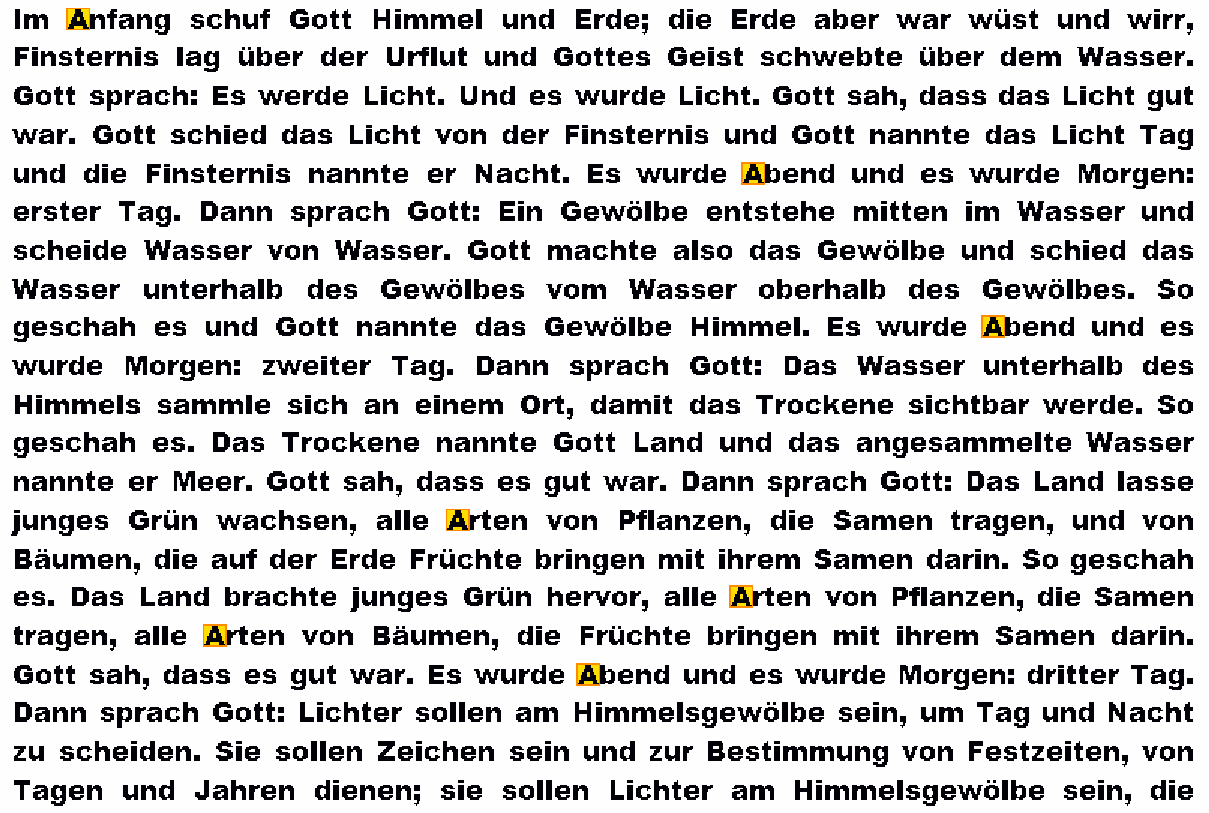
\includegraphics[width=.7\textwidth]{test-01-A}
\caption{Alle 'A' im Bild markiert.}
\label{fig:test-01}
\end{figure}

\begin{figure}[h]
\centering
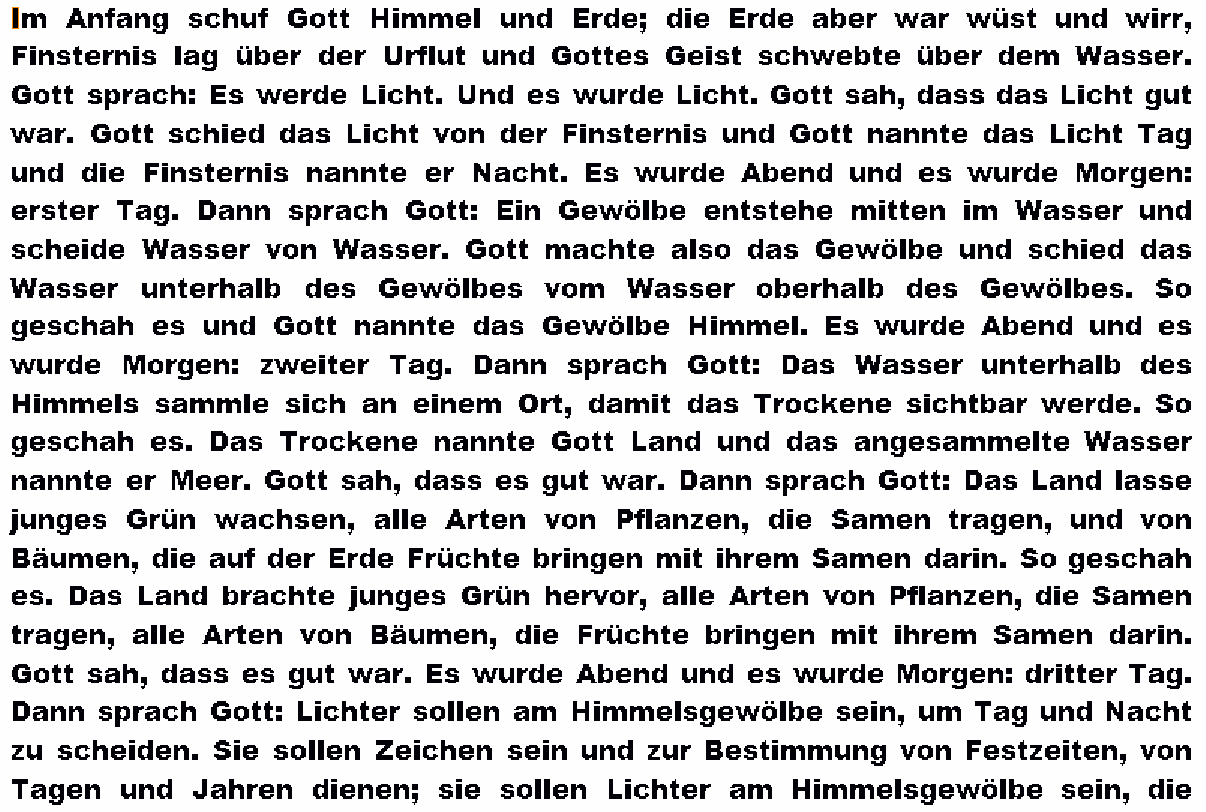
\includegraphics[width=.7\textwidth]{test-02-I}
\caption{Alle 'I' im Bild markiert.}
\label{fig:test-02}
\end{figure}

\begin{figure}[h]
\centering
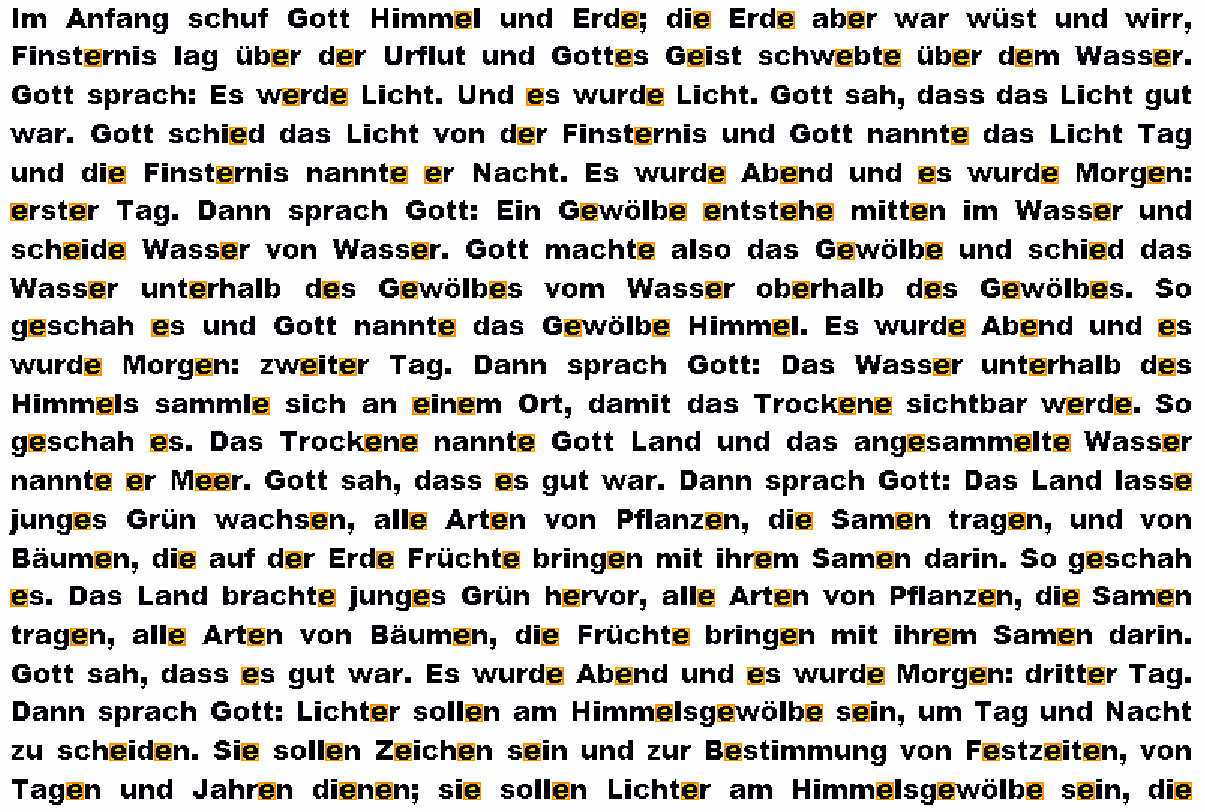
\includegraphics[width=.7\textwidth]{test-03-e}
\caption{Alle 'e' im Bild markiert.}
\label{fig:test-03}
\end{figure}

\begin{figure}[h]
\centering
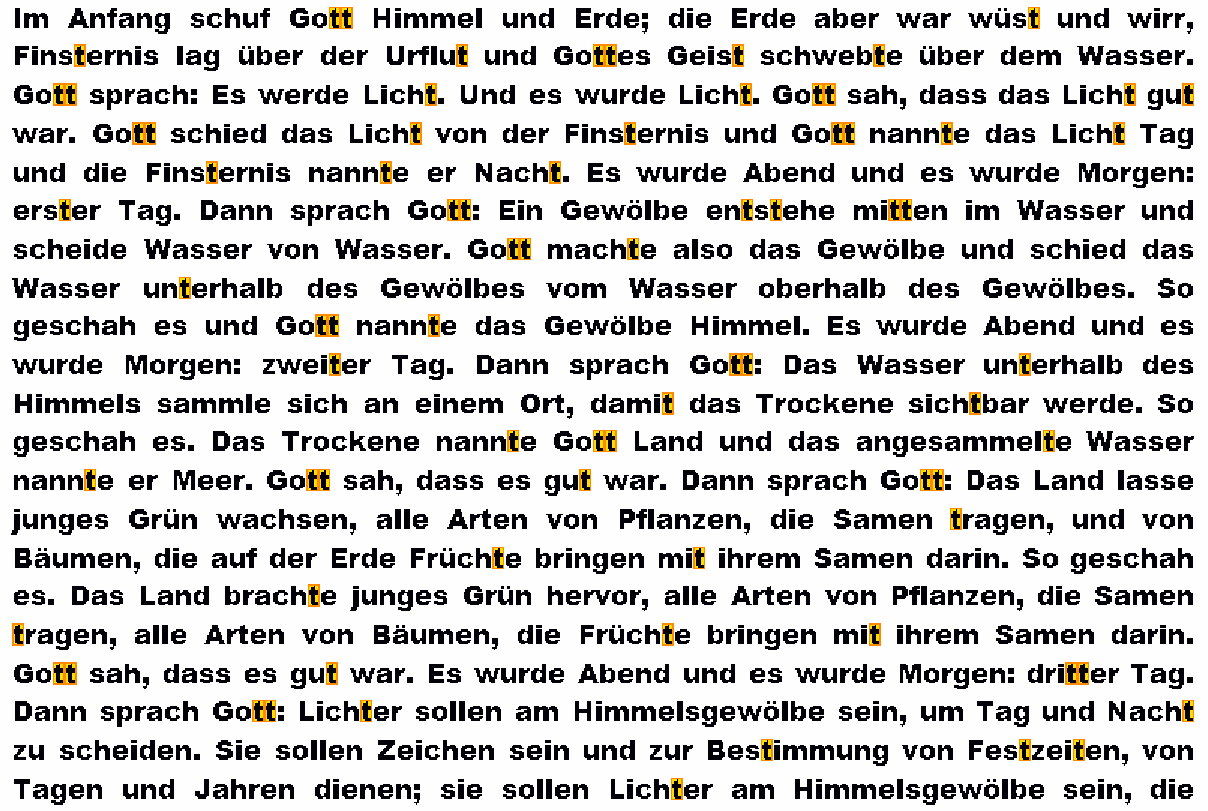
\includegraphics[width=.7\textwidth]{test-04-t}
\caption{Alle 't' im Bild markiert.}
\label{fig:test-04}
\end{figure}

\begin{figure}[h]
\centering
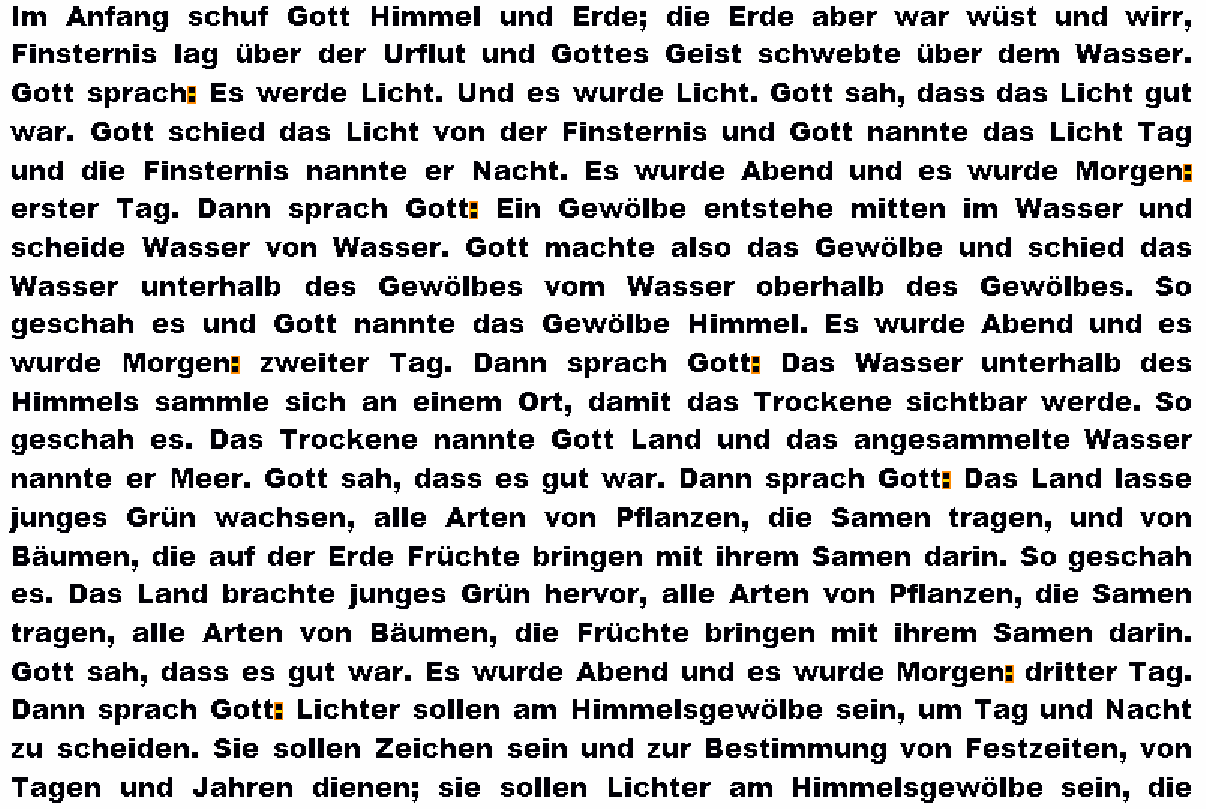
\includegraphics[width=.7\textwidth]{test-05-colon}
\caption{Alle ':' im Bild markiert.}
\label{fig:test-05}
\end{figure}

\begin{figure}[h]
\centering
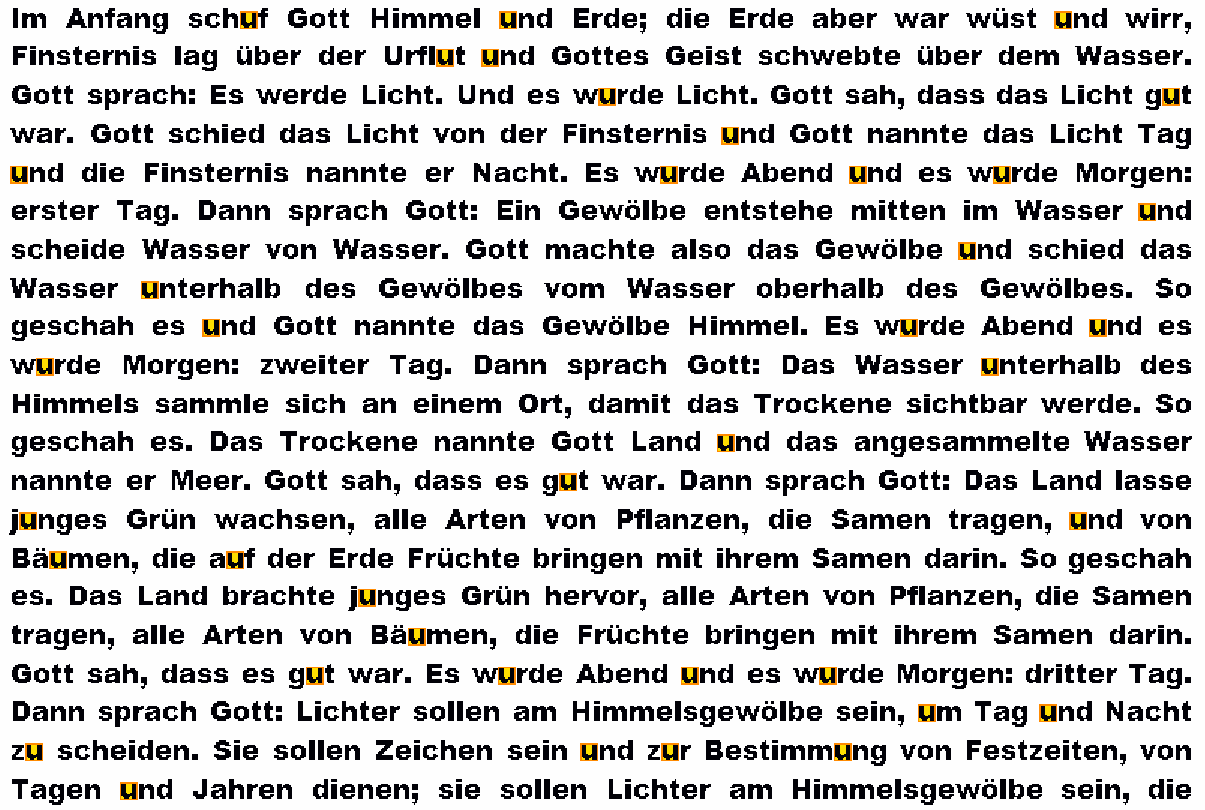
\includegraphics[width=.7\textwidth]{test-06-u}
\caption{Alle 'u' im Bild markiert.}
\label{fig:test-06}
\end{figure}

\begin{figure}[h]
\centering
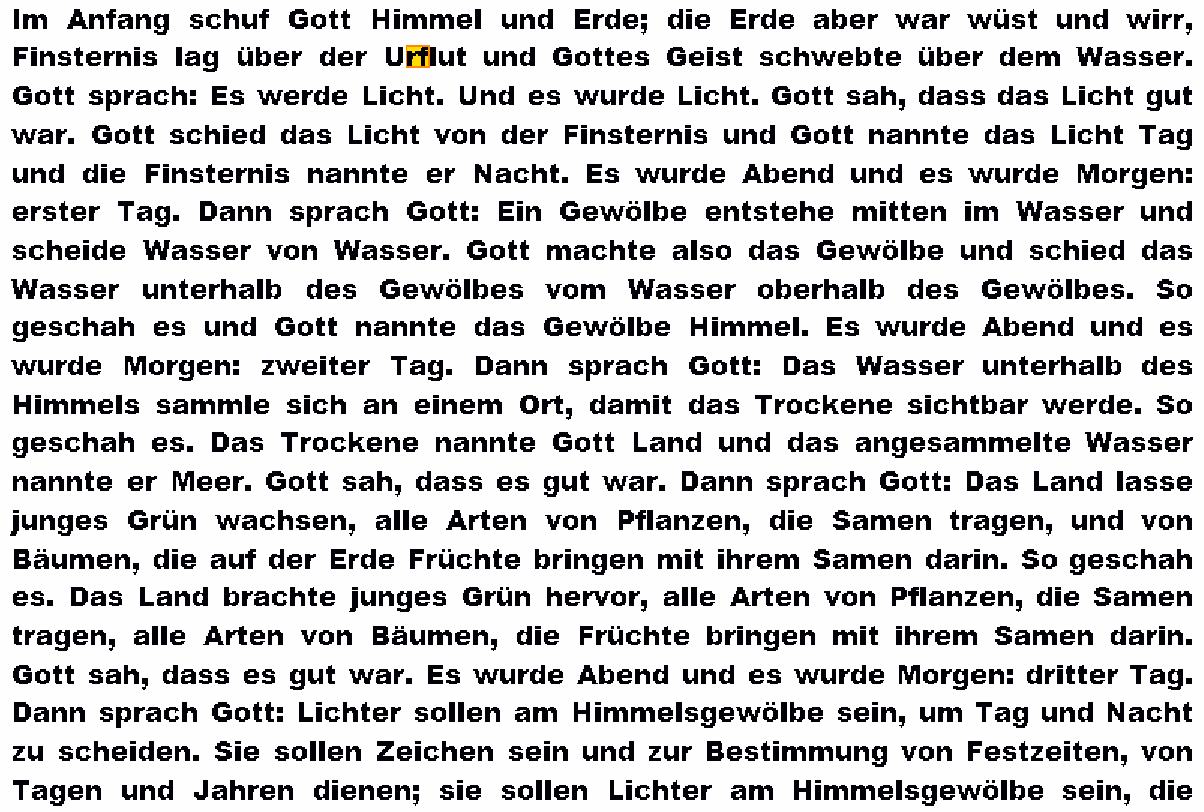
\includegraphics[width=.7\textwidth]{test-07-rf}
\caption{Alle 'rf' im Bild markiert. ('rf' wird fälschlicherweise als ein zusammenhängender Buchstabe erkannt, weil sie im Eingabe-Bild überlappend sind.)}
\label{fig:test-07}
\end{figure}


\begin{figure}[h]
    \centering\small
    \begin{tabular}{cc}
        \FramePic{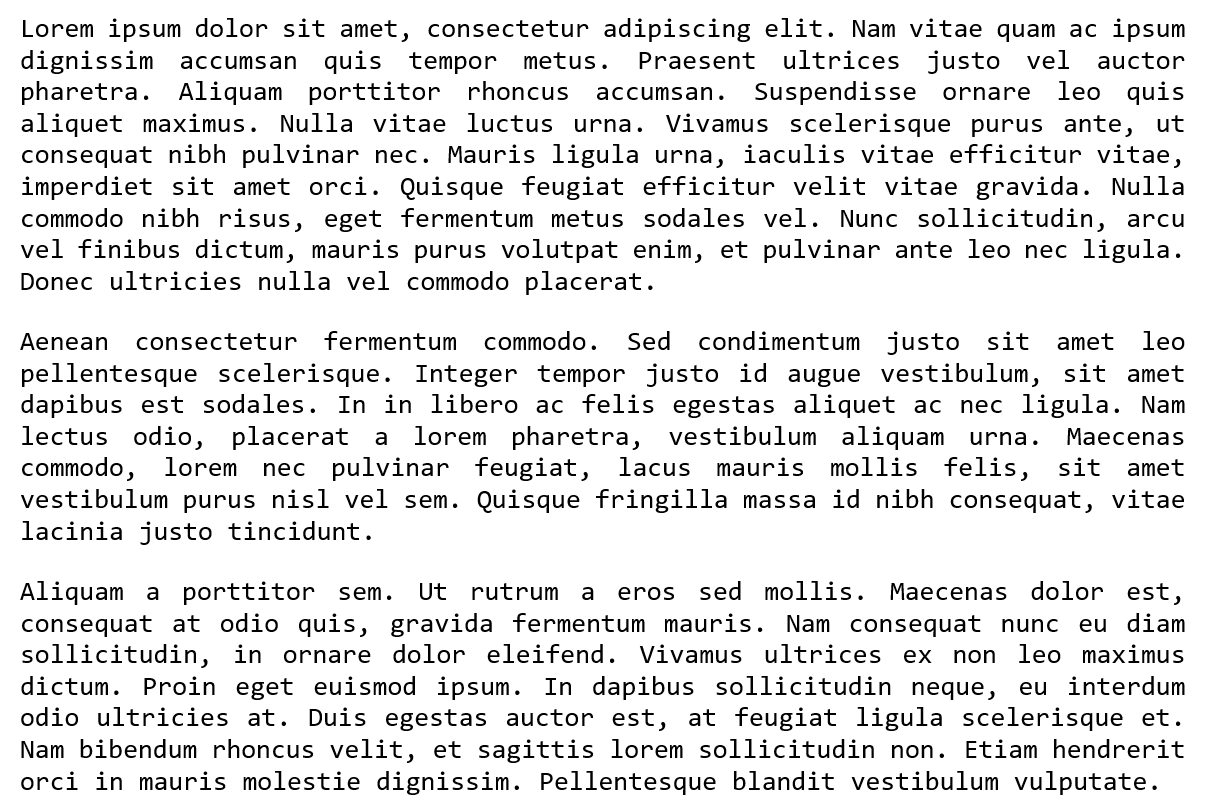
\includegraphics[width=0.5\textwidth]{consolas}} &
        \FramePic{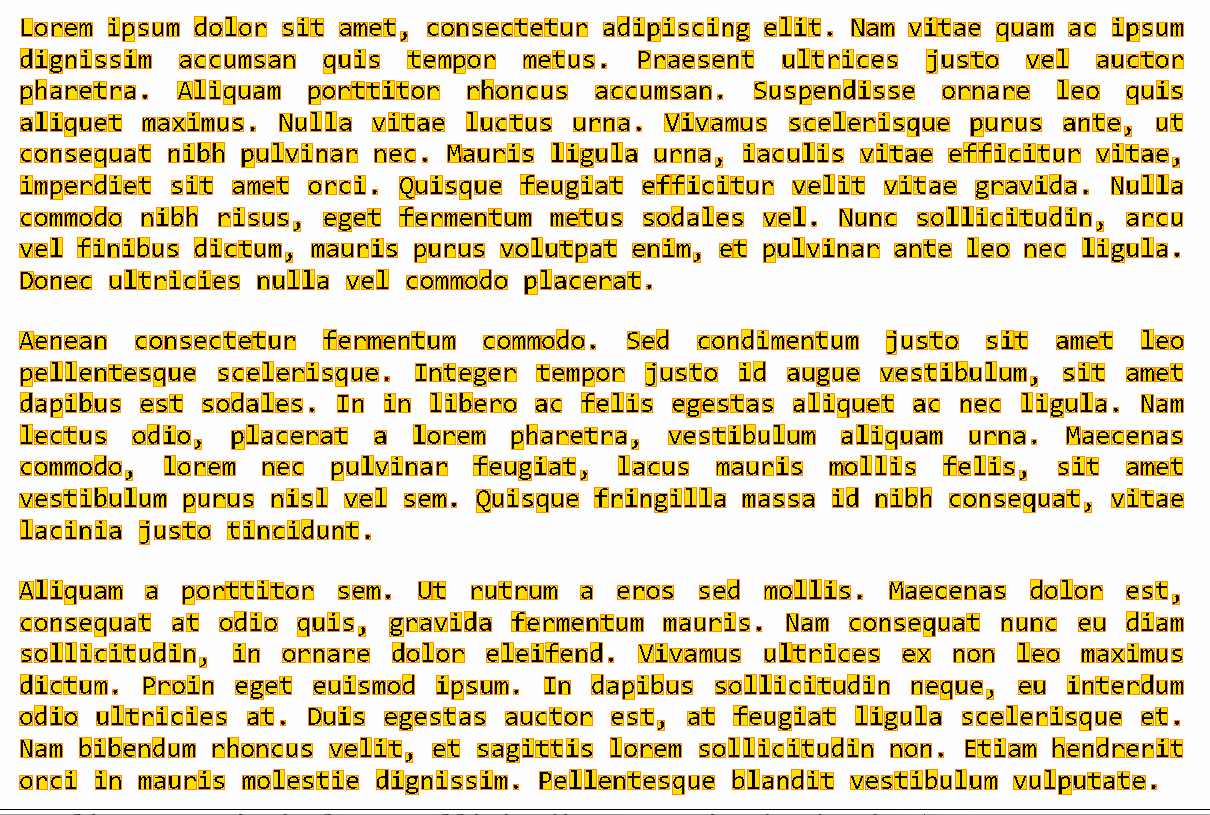
\includegraphics[width=0.5\textwidth]{test-08-consolas_mark}} \\
        (a) & (b) \\
		\FramePic{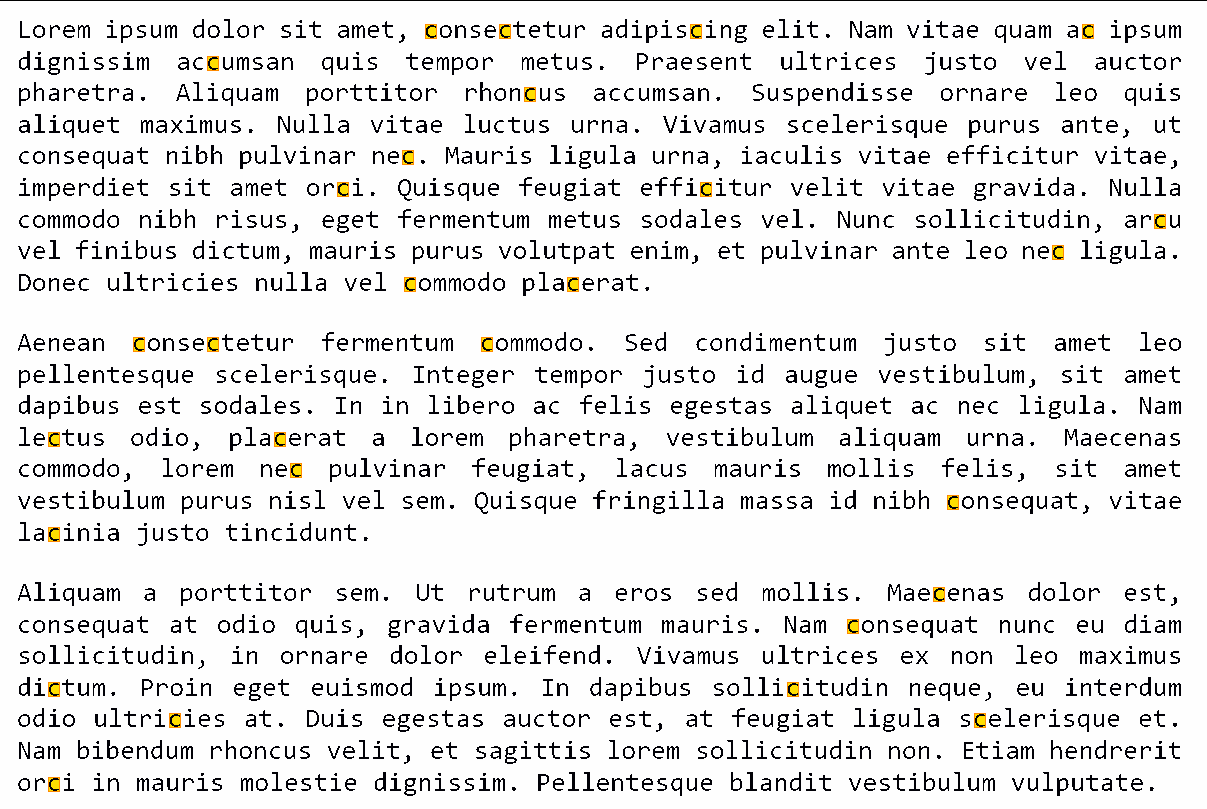
\includegraphics[width=0.5\textwidth]{test-08-consolas-c}} &
        \FramePic{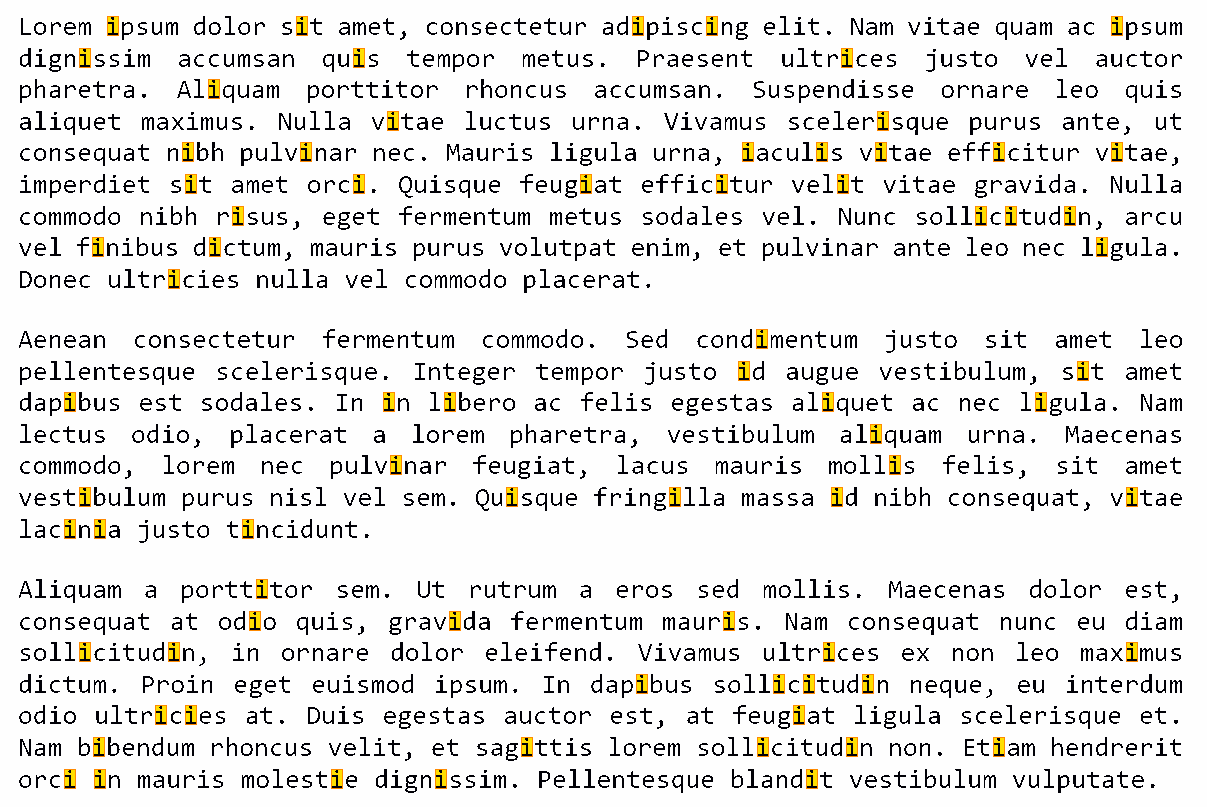
\includegraphics[width=0.5\textwidth]{test-08-consolas-i}} \\
		(c) & (d)
    \end{tabular}
    \caption{Eingabe-Bild~(a); Extrahierte Buchtaben~(b); Alle 'c' markiert~(c) sowie alle 'i' markiert~(d).}
    \label{fig:test-08}
\end{figure}

\begin{figure}[h]
    \centering\small
    \begin{tabular}{cc}
        \FramePic{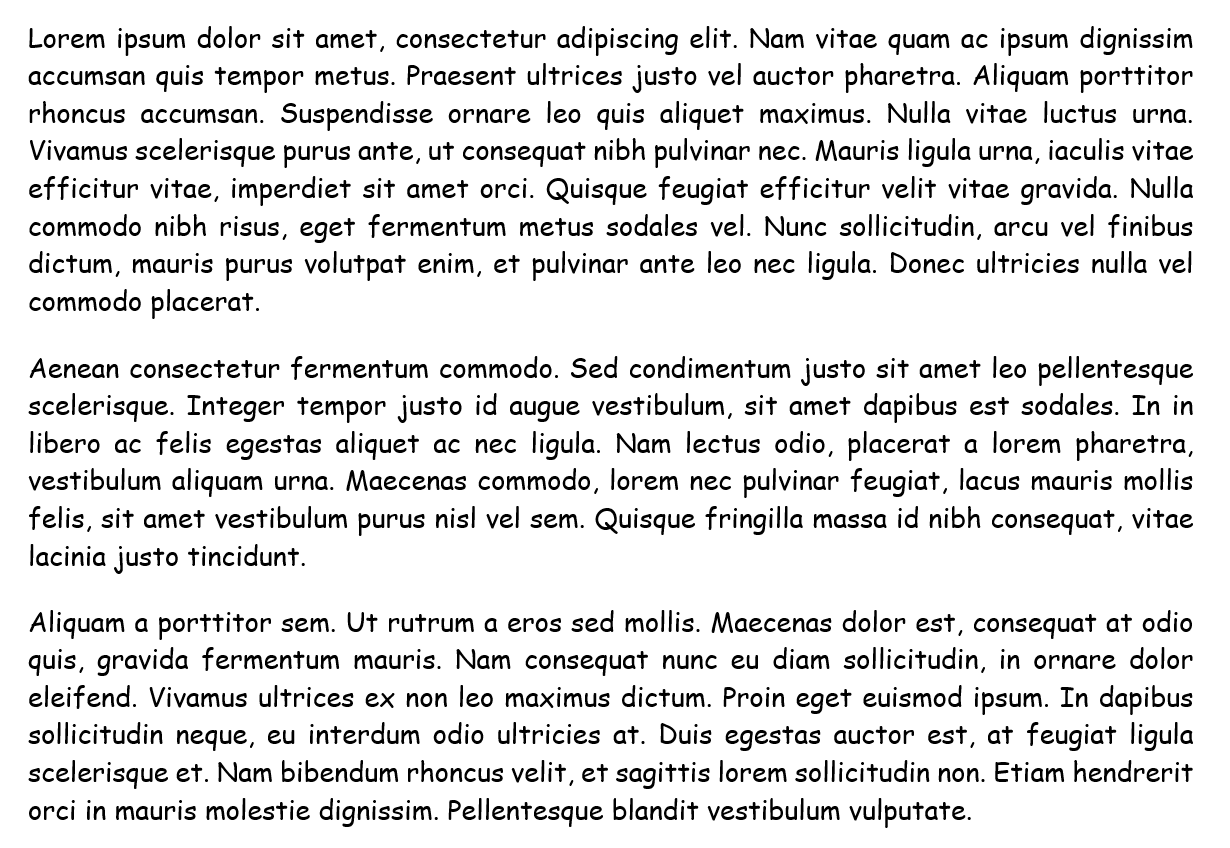
\includegraphics[width=0.5\textwidth]{comic_sans}} &
        \FramePic{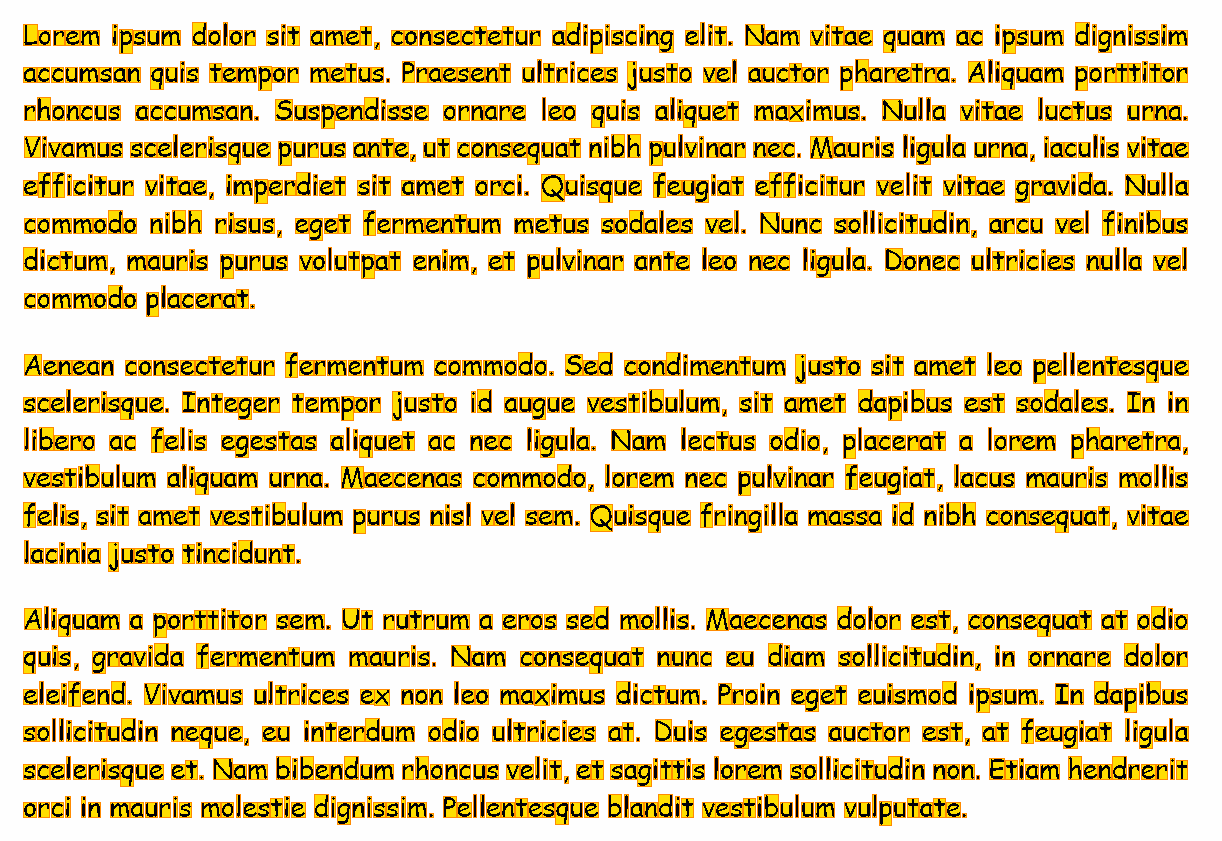
\includegraphics[width=0.5\textwidth]{test-09-comic_mark}} \\
        (a) & (b) \\
		\FramePic{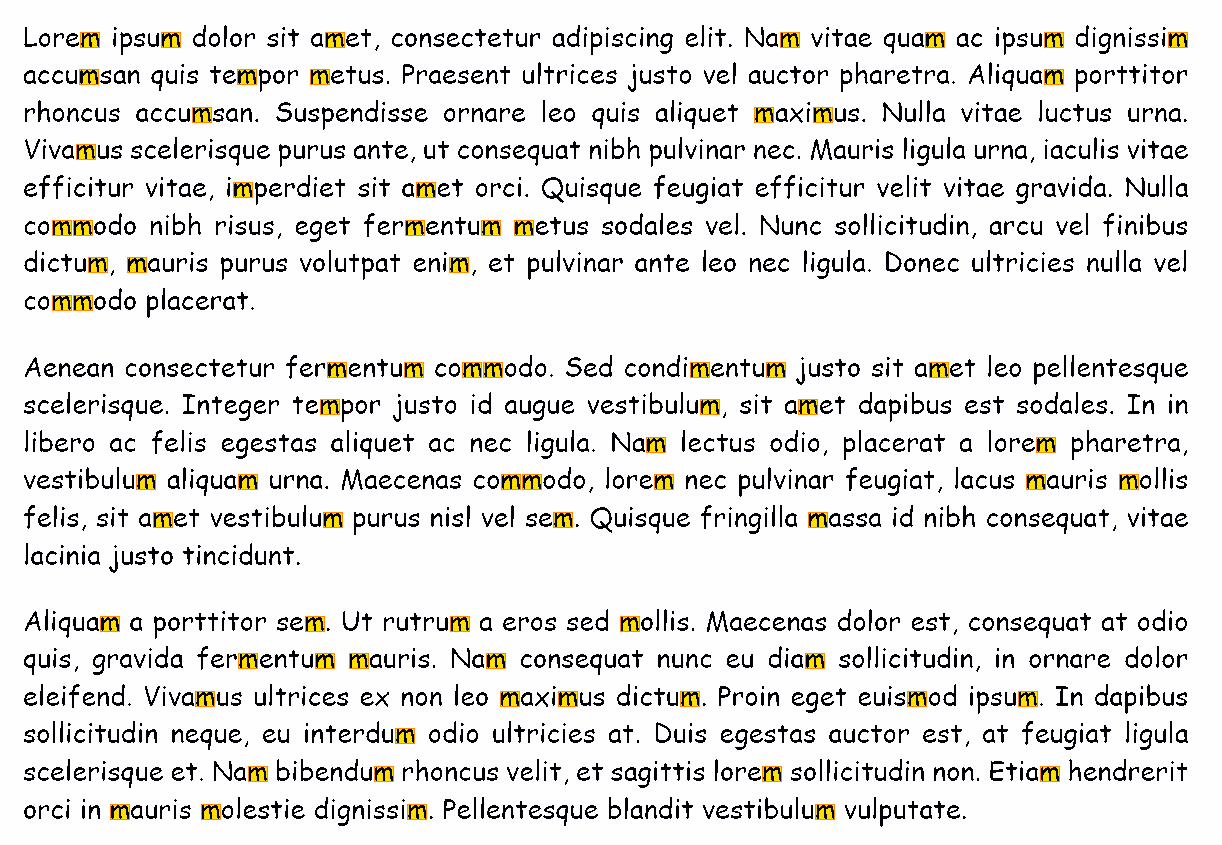
\includegraphics[width=0.5\textwidth]{test-09-comic-m}} &
        \FramePic{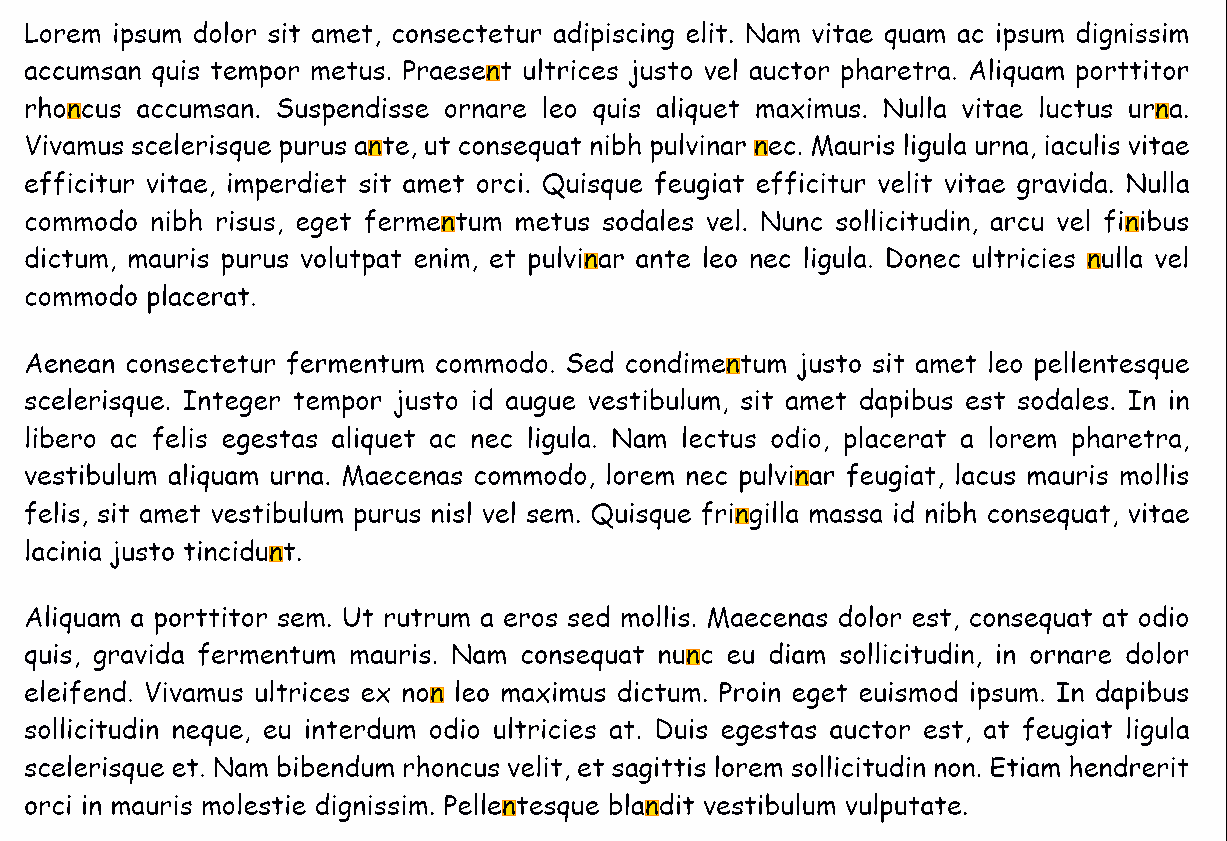
\includegraphics[width=0.5\textwidth]{test-09-comic-n}} \\
		(c) & (d)
    \end{tabular}
    \caption{Eingabe-Bild~(a); Extrahierte Buchtaben~(b); Alle 'm' markiert~(c) sowie alle 'n' markiert~(d).}
    \label{fig:test-09}
\end{figure}

\begin{figure}[h]
    \centering\small
    \begin{tabular}{cc}
        \FramePic{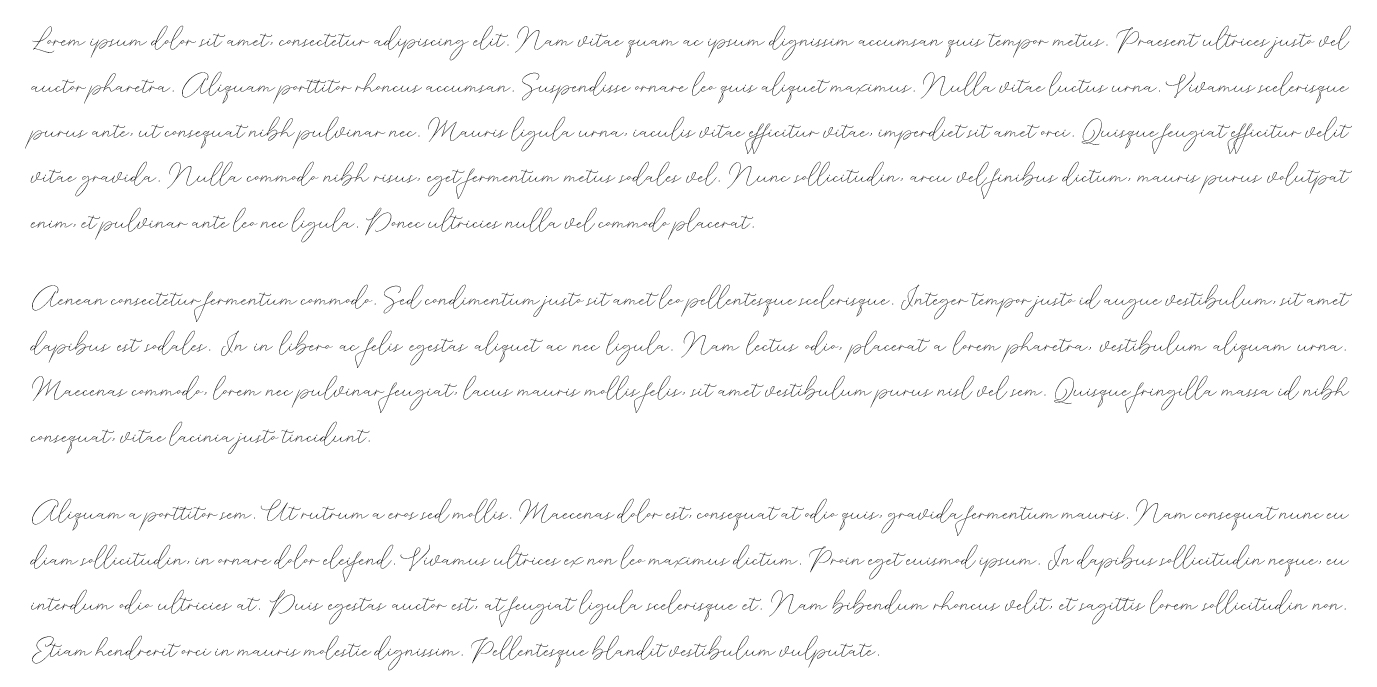
\includegraphics[width=0.5\textwidth]{Cochocib_Script_Latin_Pro}} &
        \FramePic{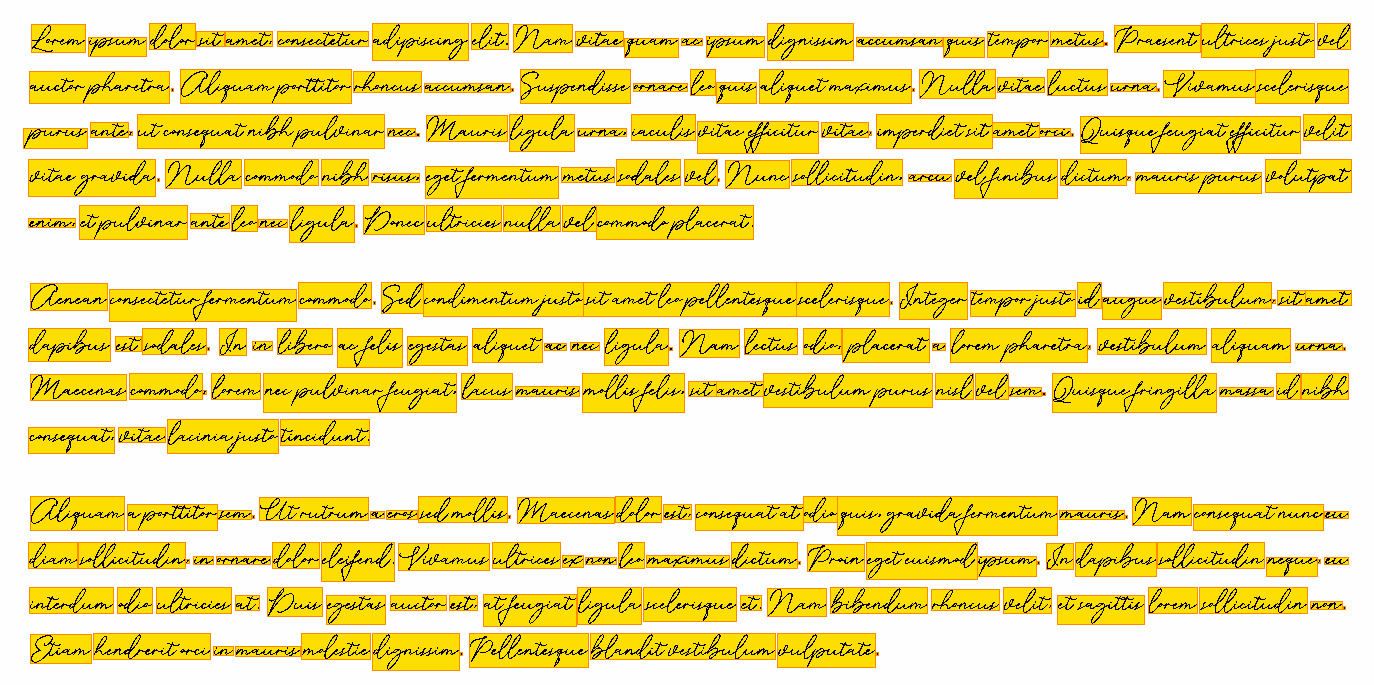
\includegraphics[width=0.5\textwidth]{test-10-cochib_mark}} \\
        (a) & (b) \\
		\FramePic{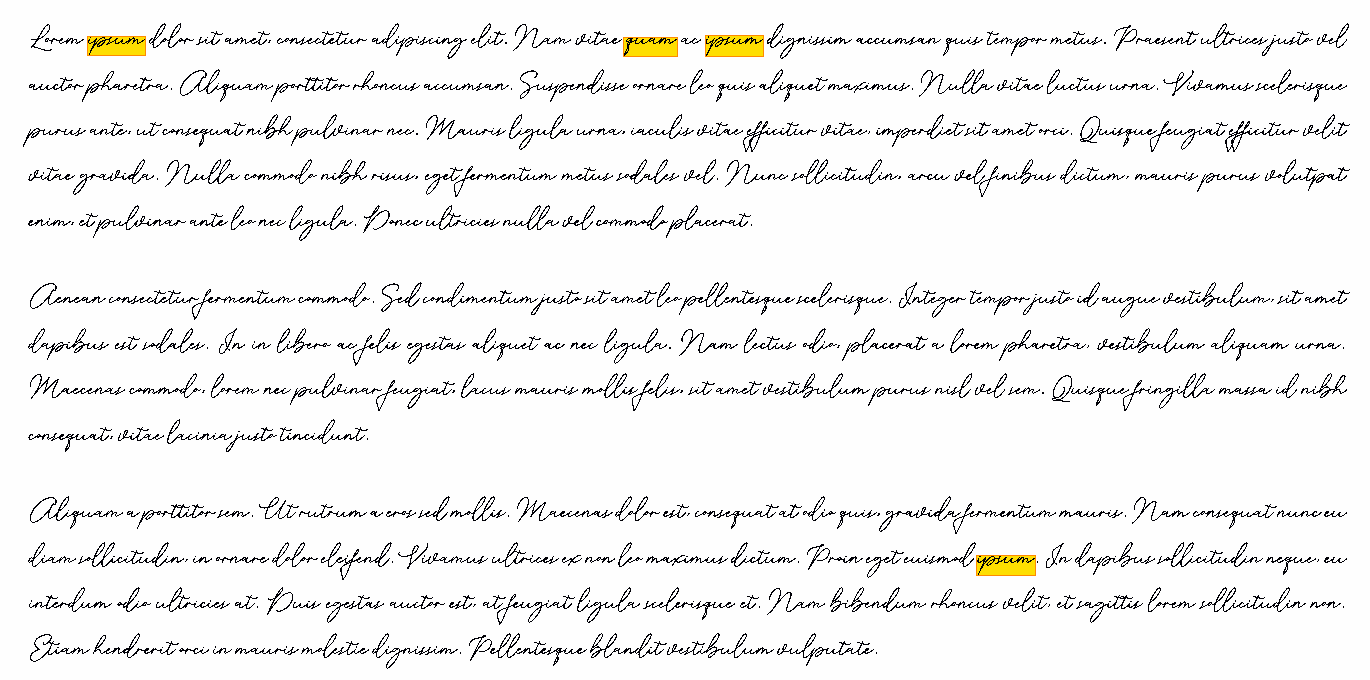
\includegraphics[width=0.5\textwidth]{test-10-cochib-ipsum}} &
        \FramePic{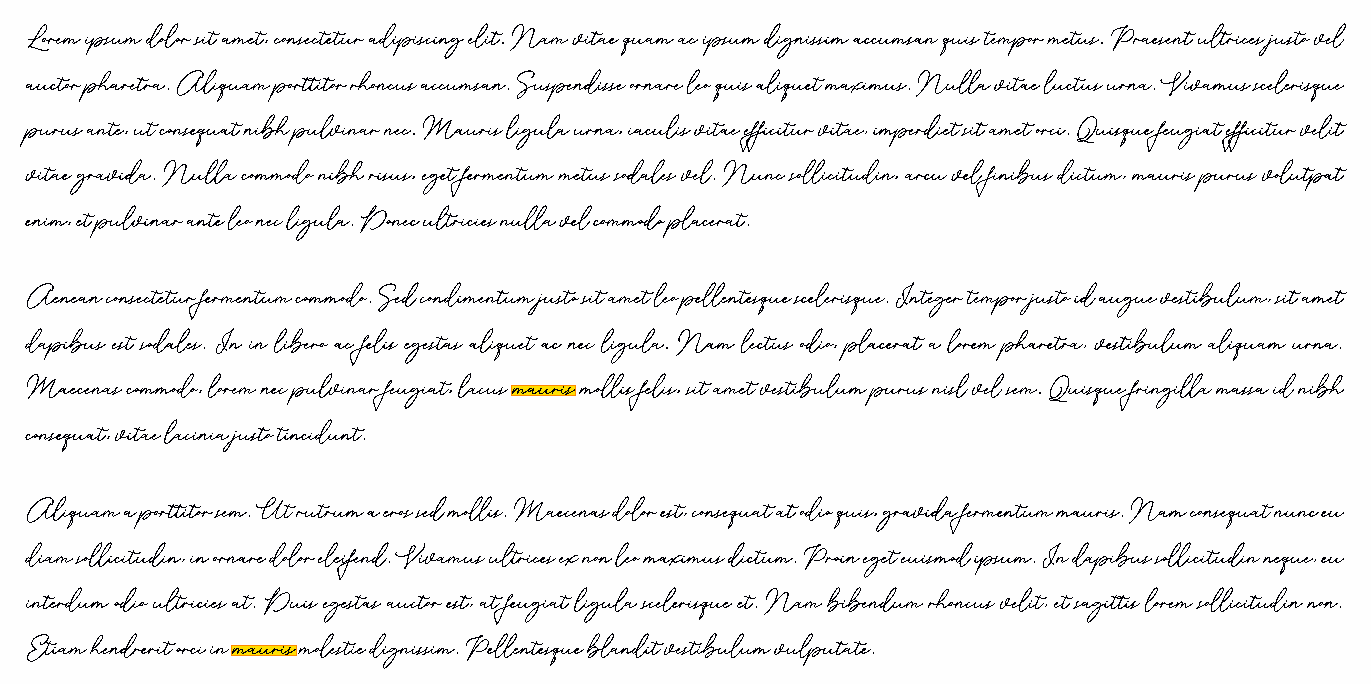
\includegraphics[width=0.5\textwidth]{test-10-cochib-mauris}} \\
		(c) & (d)
    \end{tabular}
    \caption{Eingabe-Bild~(a); Extrahierte "Buchtaben"~(b); Alle "ipsum" markiert~(c) sowie alle "mauris" markiert~(d). (Wie erwartet kommt der Algorithmus hier an seine Grenzen; durch die stark ausgeprägten Serifen werden ganze Worte als einzelne Buchstaben erkannt. Für diesen Testfall wurde der \texttt{thresholdVal} -- für die initiale Schwellenwertbildung des Graustufenbildes -- von 80 auf 220 gesetzt, weil die Schrift so "dünn" ist; für alle anderen Tests hat der Schwellenwert von 80 sehr gute Ergebnisse geliefert.)}
    \label{fig:test-10}
\end{figure}

\clearpage

\subsection{Diskussion}

\subsubsection{Welche Buchstaben können sicher erkannt werden und welche Buchstaben führen zu Problemen -- und warum?}

In den durchgeführten Tests werden alle Buchstaben sehr verlässlich erkannt; vorausgesetzt, dass die \textit{fire through} Methode nur einzelne Buchstaben liefert.

\subsubsection{Sind alle Schriftarten für diese Art von OCR-Strategie geeignet -- warum oder warum nicht?}

Es eignen sich nicht alle Schriftarten für die Erkennung mit dem implementierten Algorithmus. Es kommt zu Problemen, wenn die Schriftart Buchstabenkombinationen enthält zwischen denen es keine "Empty Column" gibt. Dies ist vorallem bei Schriftarten mit ausgeprägten Serifen der Fall.

\subsubsection{Hängt die Klassifizierungsgenauigkeit von den anderen Zeichen in der jeweiligen Zeile ab -- wenn ja, warum und wie kann dieses Problem gelöst werden?}

Wird zur Extraktion der Buchstaben \textit{fire through} ohne Post-Processing eingesetzt, dann beeinflussen die konkreten in einer Zeile auftretenden Buchstaben die Klassifizierungsgenauigkeit, weil manche Features (\zB Höhe der Bounding-Box) dadurch "verfälscht" werden.
Durch einen nachträglichen Zuschnitt der Bounding-Box oberhalb und unterhalb kann dieses Problem behoben werden. Diese Verbesserung des Algorithmus ist bereits Teil dieser Implementierung.

%%%-----------------------------------------------------------------------------

% \section{Titel der zweiten Aufgabe}

%%%-----------------------------------------------------------------------------

%\section*{Zusammenfassung und Anmerkungen}

%%%-----------------------------------------------------------------------------

% \section*{Quellen}

% \printbibliography[heading=noheader]

%%%-----------------------------------------------------------------------------
\end{document}
%%%-----------------------------------------------------------------------------